\documentclass[a4j]{jarticle}			% for platex
\usepackage[dvipdfmx]{graphicx}
\usepackage{multicol}
\usepackage{mathtools}
\usepackage{amsmath, amssymb, amsfonts}


\title{未タイトル}
\author{学籍番号 20C1119 森田大雅}
\date{\today}

\begin{document}
\maketitle % タイトルなどの出力
\small

% \twocolumnは二段組ににしない文章

\begin{abstract}
モデル図や各パラメータの説明
\end{abstract}


\begin{multicols}{2} %二段組にする


以下のようにパラメータをとる. また、この機械のモデル図が図2である.

\small
\section{手先の位置と回転角度の関係}
DH記法を用いて座標変換を行った結果、手先の位置x, y, zは以下のように求まる.
\begin{equation*}
	\left\{
		\begin{array}{c}
		\begin{split}
			&x=C_1(l_4C_{23}+l_3S_{23}+l_2S_2)\quad(3.1) \\
			&y=S_1(l_4C_{23}+l_3S_{23}+l_2S_2)\quad(3.2) \\
			&z-l_1=-l_4S_{23}+l_3C_{23}+l_2C_2\quad(3.3) \\
		\end{split}
	\end{array}
	\right.
\end{equation*}
これらの逆運動学を解くと
\tiny
\begin{equation*}
\left\{
	\begin{array}{c}
	\begin{split}
		&\theta_1=\frac{1}{2}cos^{-1}\biggl( \frac{x^2-y^2}{x^2+y^2} \biggr) \\
		&\theta_2= cos^{-1}\biggl( \frac{x^2+y^2+(z-l1)^2+l_2^2-l_3^2-l_4^2}{2l_2\sqrt{x^2+y^2+(z-l_1)^2}} \biggr)+tan^{-1}\biggl( \frac{\sqrt{x^2+y^2}}{z-l1}\biggr) \\
		&\theta_3=cos^{-1}\biggl( \frac{x^2+y^2+(z-l1)^2-l_4^2-l_3^2-l_2^2}{2l_2\sqrt{l_3^2+l_4^2}}\biggr)+tan^{-1}\biggl( \frac{-l_4}{l_3}\biggr)
	\end{split}
	\end{array}
\right.
\end{equation*}
\small

\end{multicols}

\begin{figure}[htbp]
\begin{center}
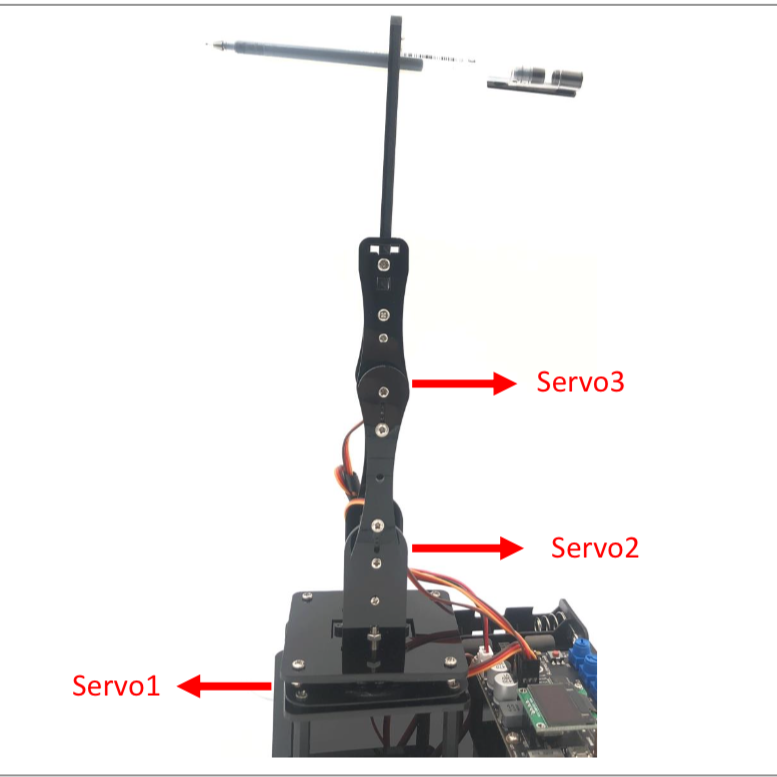
\includegraphics[width=65mm]{/home/morita/ros2_ws/Memo/tex/img/IMG_0025.PNG}
\caption{実機の写真}
\end{center}
\end{figure}

\begin{figure}[htbp]
\begin{center}
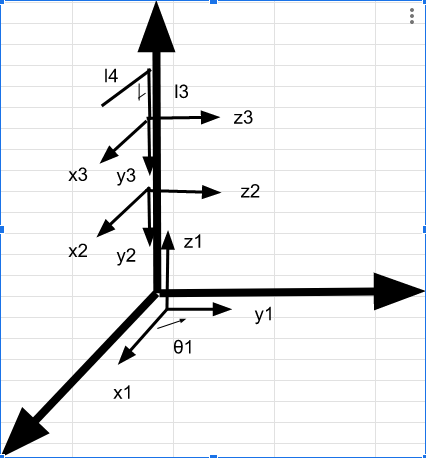
\includegraphics[width=65mm]{/home/morita/ros2_ws/Memo/tex/img/link.png}
\caption{リンク座標系}
\end{center}
\end{figure}

\begin{multicols}{2} %二段組にする

\section{参考文献}

\begin{enumerate}
\item \lbrack 1\rbrack \ Raspberry Piを利用した肖像画描画ロボット :$ \lceil Pankraz Piktograph \rfloor$ \\
\item \lbrack 2\rbrack \ XDoG: An Xtended difference-of-Gaussians compendium \\
\item \lbrack 3\rbrack \ ロボットによる描画行為の再現\\
\item \lbrack 4\rbrack \ 出版:主婦の友社\ $\lceil \text{小河原智子の似顔絵入門} \rfloor$\\
\item 広瀬\ 茂男\ 著\ 機械工学選書\ 裳華房\ ロボット工学-機械システムのベクトル解析-\\
\item 細田\ 耕著\ 実践ロボット制御-基礎から動力学まで- \\
\end{enumerate}

\end{multicols}

\end{document}
